\documentclass[12pt,a4paper]{article}
\usepackage[margin=2cm]{geometry}
\usepackage{titling}
\usepackage{graphicx}
\usepackage{subcaption}
\setlength{\droptitle}{-5em} 
\usepackage{algorithm} 
\usepackage{algpseudocode}
\usepackage{enumerate}
\usepackage{float}


\begin{document}
\title{\huge \textbf{Overall Software Plan} \\ \LARGE {\textbf{CS 346: Assignment-2A}}}
\author{\Large Group 10-A}
\date{210101113-210101119}
\maketitle


\section{Problem Statement}
(Yashraj)
    
    
\section{Software Requirements and Assumptions}
The following are the specifications of the software that has to be developed that has been mentioned in the problem statement: (Agrawal)
\begin{itemize}
    \item Item1
    \item Item2
\end{itemize}

\section{Data Flow Diagrams}
Short Desc (Yashraj) \textbf{Bold}, \texttt{Verb}, \textit{Italics}
\subsection{Level-0 DFD}
(Yashraj)
\subsection{Level-1 DFD}
(Yashraj)

\subsection{Level-2 DFDs}
The following subsections highlight the detailed \textbf{Level-2} Dataflow diagrams of various processes in the Academic system Management software:
\subsubsection{Admission Management Process}
(Gupta)
\subsubsection{Course Management Process}
(Tanish)
\subsubsection{Examination Management Process}
(Pratyush)
\subsubsection{Grade Management Process}
(Dhanesh)
\subsection{Entity Relationship Diagram}
(Ketan)

\subsection{Feature Enhancement}
(Shivam)
\begin{itemize}
    \item hrtrt
    \item rtrtrtrttrt
\end{itemize}
        
\section{User Interface}
(Shivam Agrawal)
	The user interface for this software can be developed using \texttt{Visual Basic}. The following are the tentative list of toolbox components needed for the basic implementation (without any feature enhancement):
    \begin{itemize}
        \item \textbf{Text Box:} sdfeerererererer
        \item And so on....
    \end{itemize}

    \subsection{Basic Design}
    This is the tentative basic design of the user interface which is to be designed in \textbf{Visual Basic} using the components listed above:
    \begin{figure}[h]
        \centering
        \begin{subfigure}[b]{0.45\linewidth}
            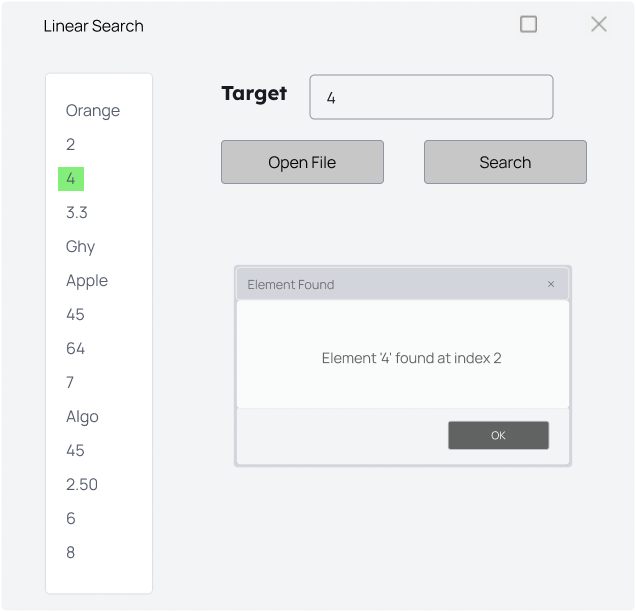
\includegraphics[width=\linewidth]{Prototype.png} 
            \caption{Message box output when element is found.}
            \label{fig:sub1}
        \end{subfigure}
        \hfill
        \begin{subfigure}[b]{0.45\linewidth}
            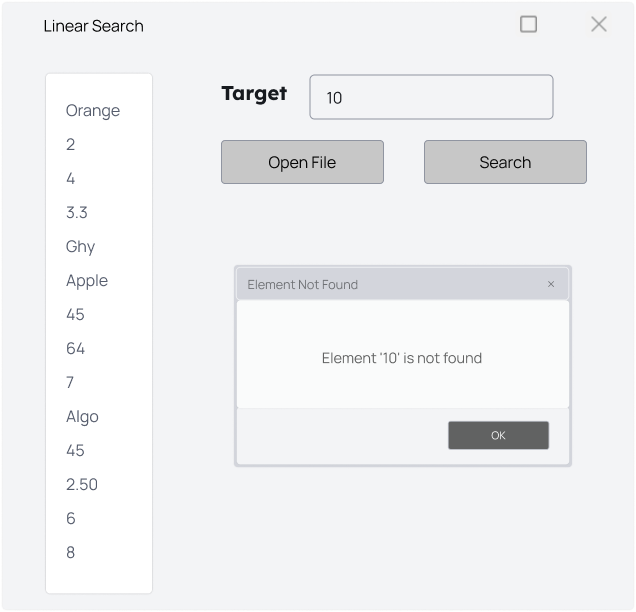
\includegraphics[width=\linewidth]{Prototype-2.png}
            \caption{Message box output when element is not found.}
            \label{fig:sub2}
        \end{subfigure}
        \caption{Basic design of the software application}
        \label{fig:overall}
    \end{figure}
\subsection{Subsections}
\end{document}